\frame{
\section{Lavoro}
\subsection[Modello]{Parte I. Modellazione della deambulazione}
\frametitle{Raccolta e morfologia dei dati}
\scriptsize{
\begin{table}[htbp]
	\centering
	\rowcolors{1}{RoyalBlue!20}{RoyalBlue!5}
	\begin{tabular}{l|c}
			Attivit�& cammino \\
			Soggetti& $6$ \\
			Velocit�& $\{3,4,5,6,7\}\,km/h$\\
			Durata& $2\, minuti$ per attivit�\\
			Strumenti & IMU, Vicon, tappeto rullante\\
			Luogo& Laboratorio\\
			Dati raccolti & valori giroscopio monoassiale\\
			Freq. camp & $100\, Hz$
		\end{tabular}
	\label{tab:TabellaRiassuntivaRaccoltaDati}
\end{table}
}



\begin{figure}
\centering
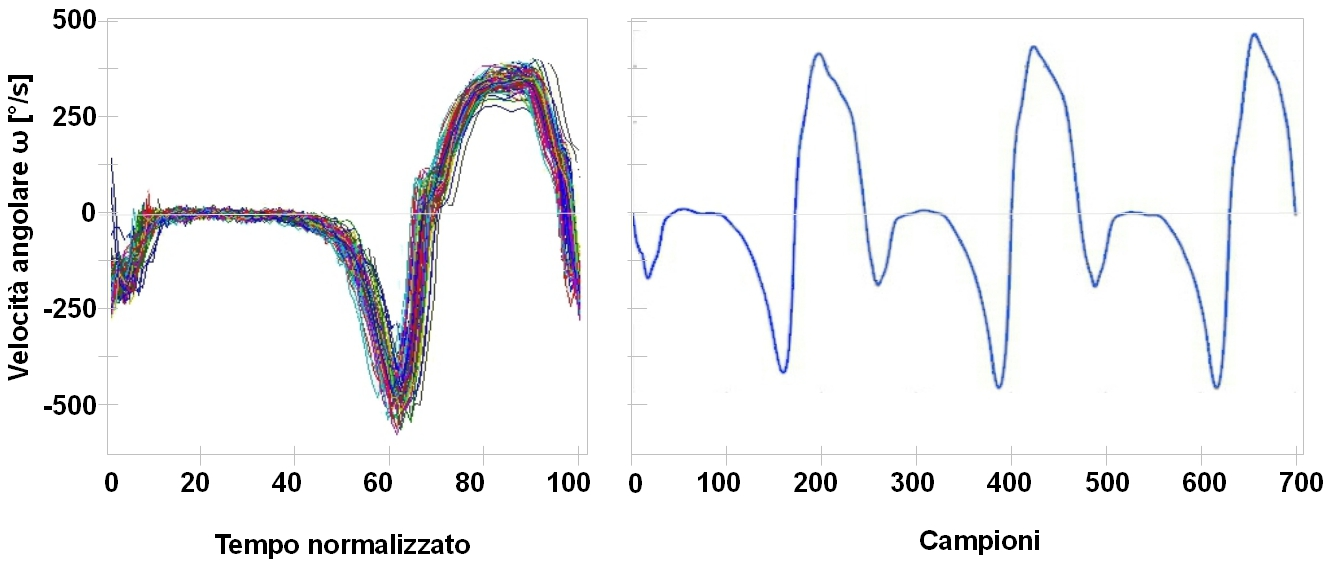
\includegraphics[width=.95\textwidth]{imgs/gyroSignal.jpg}
\end{figure}
} 





\frame{
\begin{figure}
%\frametitle{Parte I. HMM per l'analisi della deambulazione}
\frametitle{HMM per l'analisi della deambulazione}
\centering
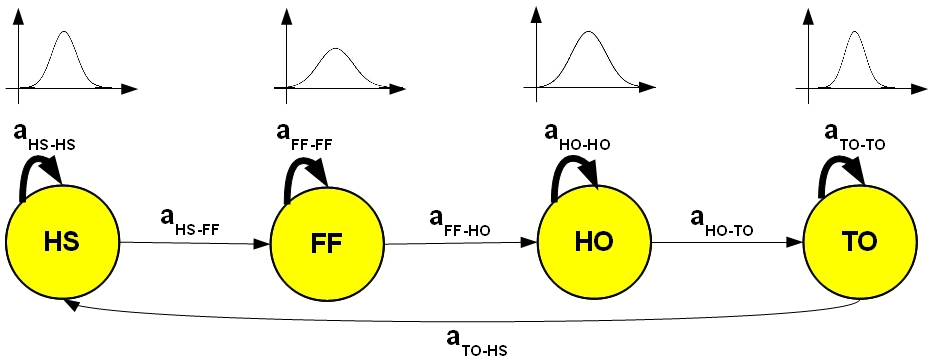
\includegraphics[width=.95\textwidth]{imgs/HMM.jpg}
\end{figure}
\begin{block}{HMM minimale}	
\begin{itemize}
\begin{columns}
\column{.4\textwidth}
	\item $S = \{HS, FF, HO, TO\}$
	\item Sinistra-Destra ciclico 
		\[
			a_{ij} > 0 \Leftrightarrow \left\{
			\begin{array}{l}
				j = i \\
				j = i+1 \\
				i = N \;\text{e}\; j = 1
			\end{array}
		\]

\column{.5\textwidth}
	\item Emissioni gaussiane monovariate $b_j(x) = \mathcal{N}(x,\mu_j,\sigma_j) = \frac{1}{\sigma_j\sqrt{2\pi}}\textbf{e} ^{-\frac{(x-\mu_j)^2}{2\sigma_j^2}}$
	\end{columns}
\end{itemize}
\end{block}
}  




\frame{
\frametitle{Addestramento e validazione modello (1/2): etichettamento}
\begin{columns}[c]
\column{.4\textwidth}
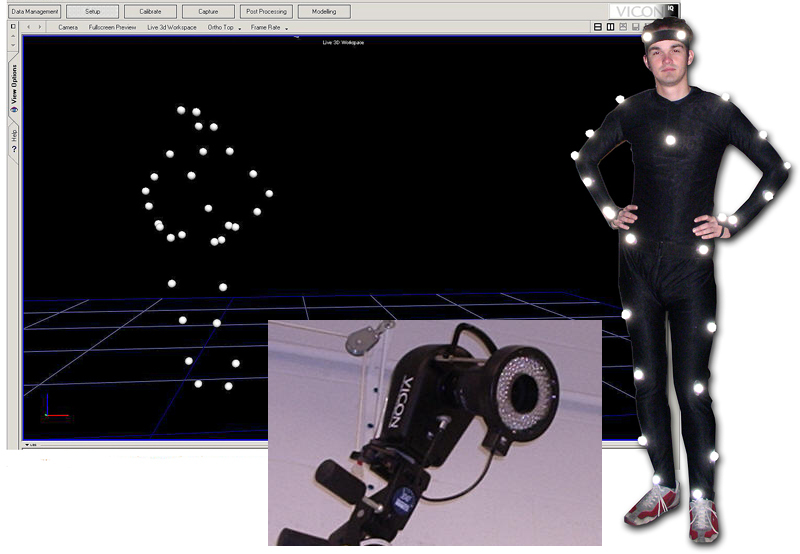
\includegraphics[width=1\textwidth]{imgs/viconMotionCapture.jpg}
\column{.7\textwidth}
\centering
	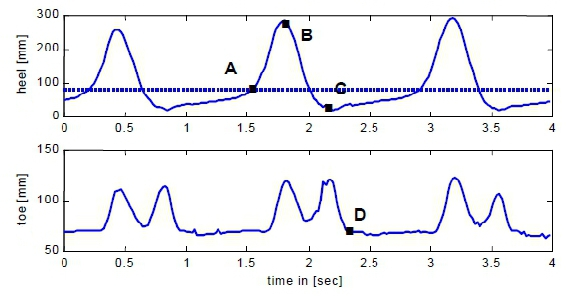
\includegraphics[width=1\textwidth]{imgs/ViconMeasurementsPappas.jpg}


\end{columns}
\begin{block}
\tiny{
\begin{itemize}
	\item $\pi_i = N_i/N_{tot}$
	\item $a_{ij} = $ 
		$
			 \left\{
			\begin{array}{l}
				C/N_i   \quad  \text{se}\quad j = (i+1)\%Q \quad C \,\text{cicli deambulazione nel \textit{Training Set}}\\
				1- C/N_i\quad  \text{se} \quad j = i\\
				0       \quad  \text{altrimenti}
			\end{array}
	$
	\item $b_i(\Omega(t))=$
				$\left\langle \mu_i = \dfrac{1}{N_i} \displaystyle \sum_{t=1}^T{\Omega(t)},\quad
				\sigma_i = \sqrt{\dfrac{1}{N_i -1}\displaystyle \sum_{t=1}^T({\Omega(t)-\mu_i})^2} \right\rangle$
\end{itemize}
}
\end{block}
} 

 
\frame{
\frametitle{Addestramento e validazione modello (2/2): \textit{leave} \textit{one} \textit{subject} \textit{out} \textit{cross} \textit{validation}}
\begin{block}{Validazione della capacit� di generalizzazione del modello}
\centering
	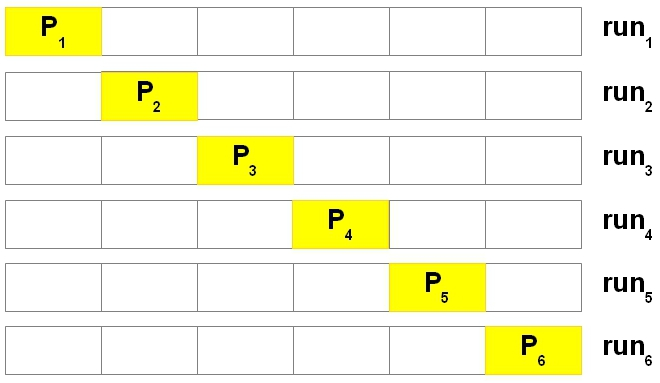
\includegraphics[width=.7\textwidth]{imgs/LOOCV.jpg}
\end{block}
}

\frame{
%
\frametitle{La segmentazione}
\begin{block}{Algoritmo di Viterbi}
Data $\left\langle HMM, O\right\rangle$, la decodifica restituisce sequenza pi� probabile di stati $S^*$. 
\begin{enumerate}
	\item Fase \textit{Forward}: costruzione di sequenze parziali a probabilit� massima
	\item Fase \textit{Backtracking}: calcolo a ritroso della sequenza pi� probabile
\end{enumerate}
\end{block}

\begin{columns}
\column{.5\textwidth}
\begin{block}{Problema}
\textit{Backtracking} non in linea
\end{block}
\column{.5\textwidth}
\begin{block}{Soluzione}
\textit{Short-Time Viterbi} Bloit-Rodet 2008 \cite{short_time_viterbi_online_hmm_deconding}\\
\end{block}
\end{columns}

\begin{block}{Funzionamento Viterbi in linea}
\begin{enumerate}
	\item creazione di una finestra temporale $[a,b]$ 
	\item applicazione Viterbi solo fase \textit{Forward} 
	\item \textit{Backtracking} da ciascuno stato finale 
	\item le sequenze da $a$ fino a $\tau \;(\tau \leq b)$ combaciano $\Rightarrow$ segmentazione 
	\begin{itemize}
		\item spostamento finestra $a = a + \tau$ e $b = a + 1$ e fase (2)
	\end{itemize}
	\item altrimenti
	\begin{itemize}
		\item allargamento finestra $b = b + 1$ e fase (2)
	\end{itemize}
\end{enumerate}
\end{block}
}


%%%%%%%%%%%%%%%%%%%%%%%%%%%%%%%%%%%%%%%%%%%%%%%%%%%%%%%%%%%%%%%%%%%%%%%%%%%%%%%%%%%%%%%%%%%%%%%%%%%%%%%%%%%%%%%%%%%%%%%%%
%%%%%%%%%%%%%%%%%%%%%%%%%%%%%%%%%%%%%%%%%%%%%%%%%%%%%%%%%%%%%%%%%%%%%%%%%%%%%%%%%%%%%%%%%%%%%%%%%%%%%%%%%%%%%%%%%%%%%%%%%
\frame{\subsection[Android app]{Parte II. Applicazione Android\tm}
\frametitle{Architettura dell'applicazione}
\begin{center}
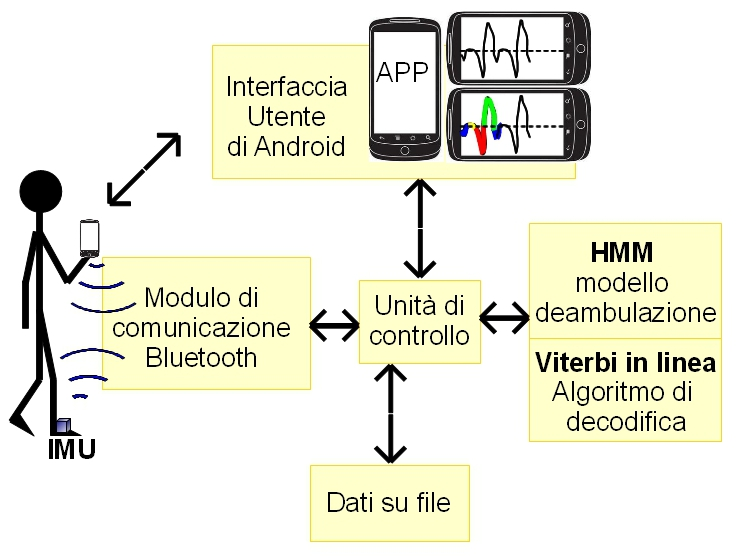
\includegraphics[width=.8\textwidth]{imgs/ArchitetturaProgramma.jpg}
\end{center}
} 


\frame[containsverbatim]{
\frametitle{Interfaccia utente}

\begin{center}
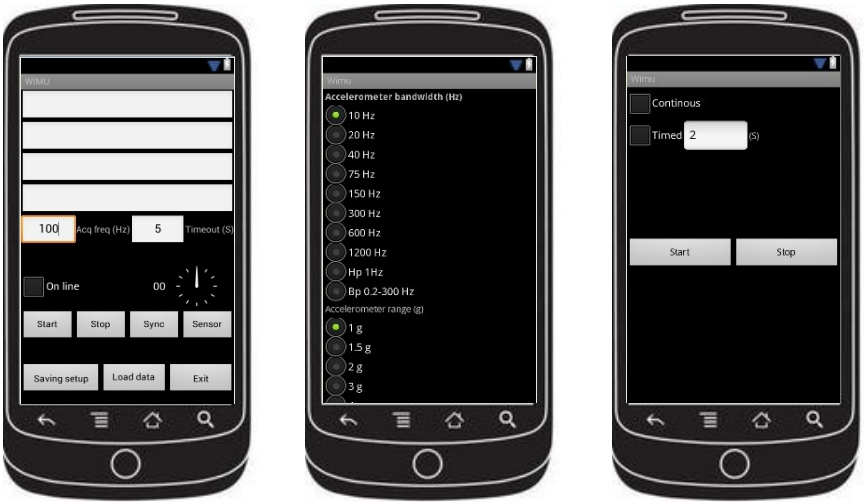
\includegraphics[width=.8\textwidth]{imgs/UI.jpg}
\end{center}
\begin{columns}
\column{.45\textwidth}
\begin{block}{Criteri di programmazione}
\begin{itemize}
	\item semplicit�
	\item classe \verb|Activity|
	\item programmazione a eventi
\end{itemize}
\end{block}
\column{.5\textwidth}
\put(-20,0){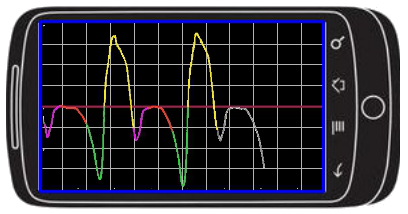
\includegraphics[width=.9\textwidth]{imgs/SegmentationAndroid.png}}
\end{columns}
}


\frame[containsverbatim]{
%\frametitle{Parte II. Applicazione Android\tm: gestione processi}
\frametitle{Gestione processi, Comunicazione}
\begin{block}{Thread e Android: massima reattivit� (5s di blocco tollerato)}
\begin{itemize}
	\item \textit{UI-thread} (main) delega operazioni lunghe o potenzialmente bloccanti. 
	\item Asincrono: un \textit{task} viene eseguito da \textit{worker thread} ed il risultato viene pubblicato sullo \textit{UI-thread} mediante \verb|Handler|
%	A Handler allows you to send and process Message and Runnable objects associated with a thread's MessageQueue. Each Handler instance is associated with a single thread and that thread's message queue. When you create a new Handler, it is bound to the thread / message queue of the thread that is creating it -- from that point on, it will deliver messages and runnables to that message queue and execute them as they come out of the message queue.

	
\end{itemize}
\end{block}

\begin{block}{Comunicazione}
\begin{itemize}
	\item \verb|Intent|: sistema di messaggistica per \verb|Activity| ed altri componenti
	\item \verb|Application|: stato globale dell'applicazione
\end{itemize}
\end{block}
}

\frame{
\frametitle{Implementazione HMM e Viterbi in Java - Android\tm}
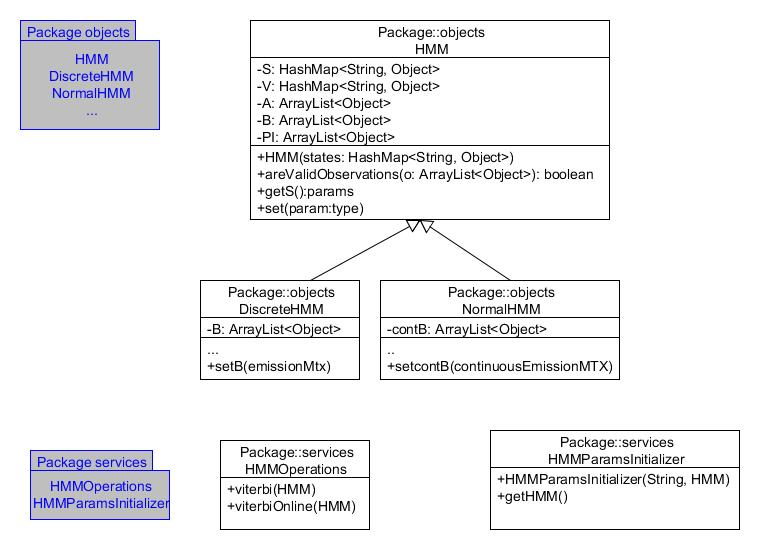
\includegraphics[width=.95\textwidth]{imgs/HMMuml.jpg}\\
}


\frame{
\subsection{Parte III. Valutazione}
%\frametitle{Parte III. Valutazione delle prestazioni del sistema}
\frametitle{Valutazione delle prestazioni del sistema}
\begin{columns}
\column{.5\textwidth}
%\putat{100}{-110}{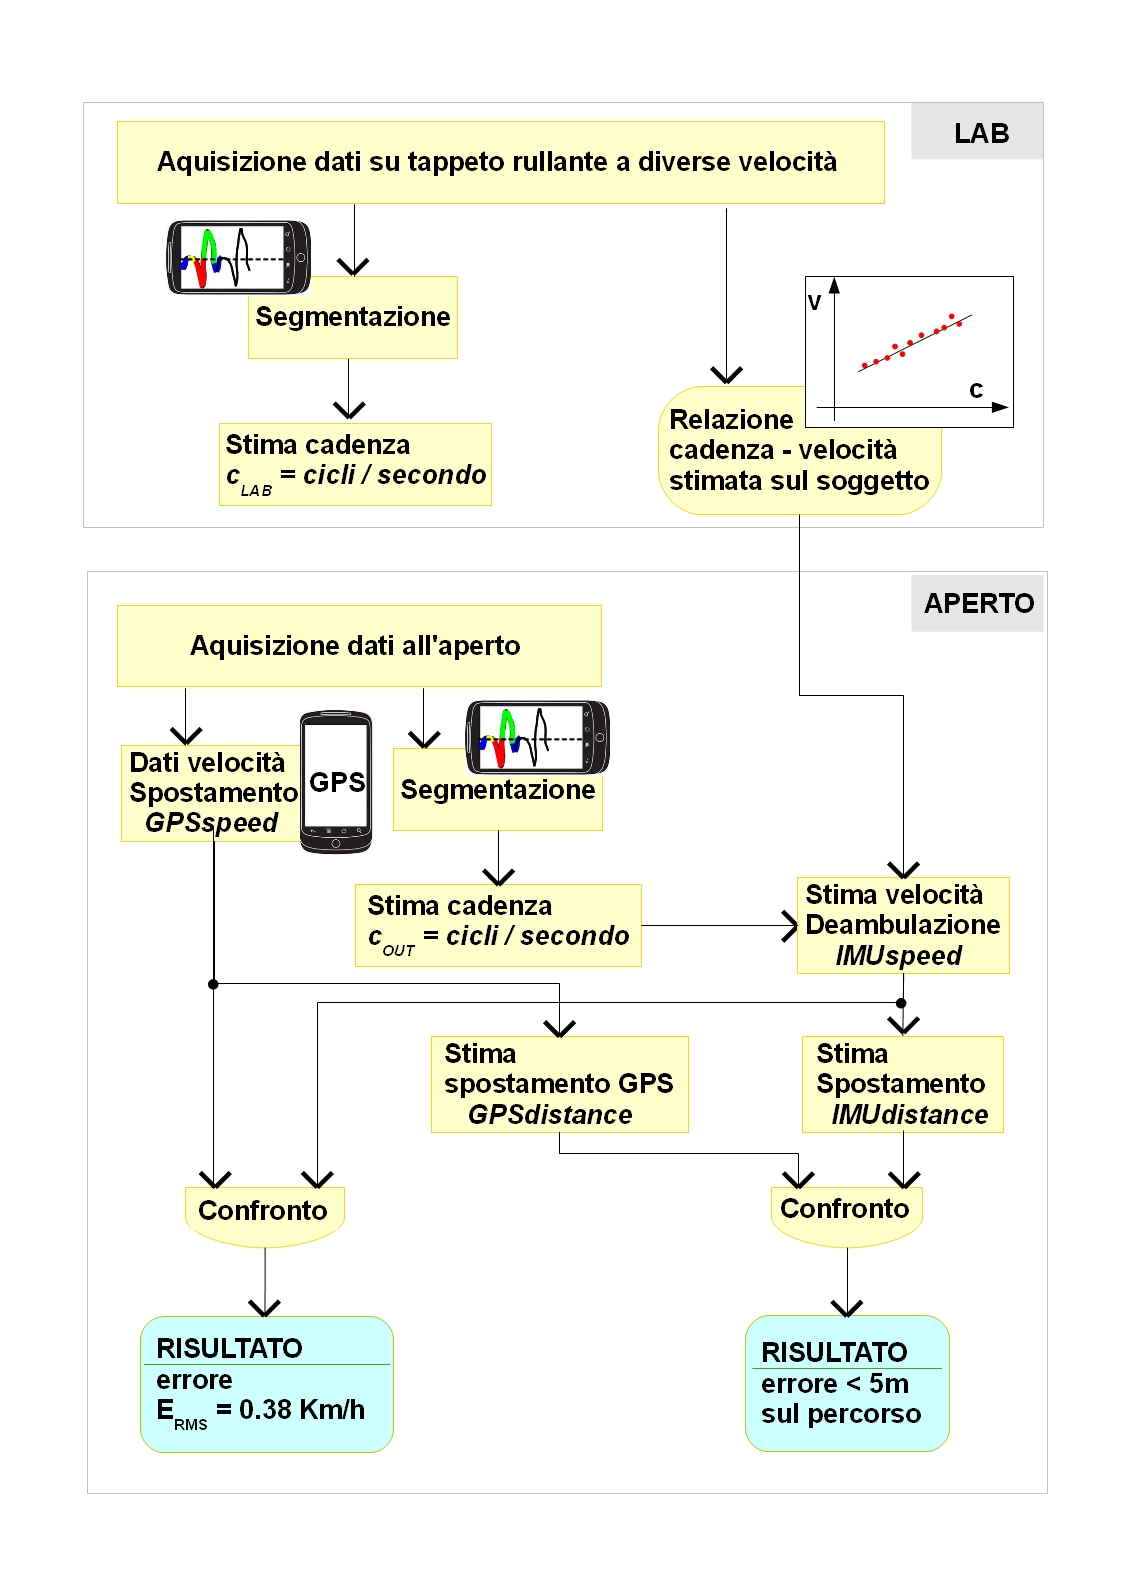
\includegraphics[width=1\textwidth]{imgs/ValutazionePrestazioniSistema.jpg}}\\
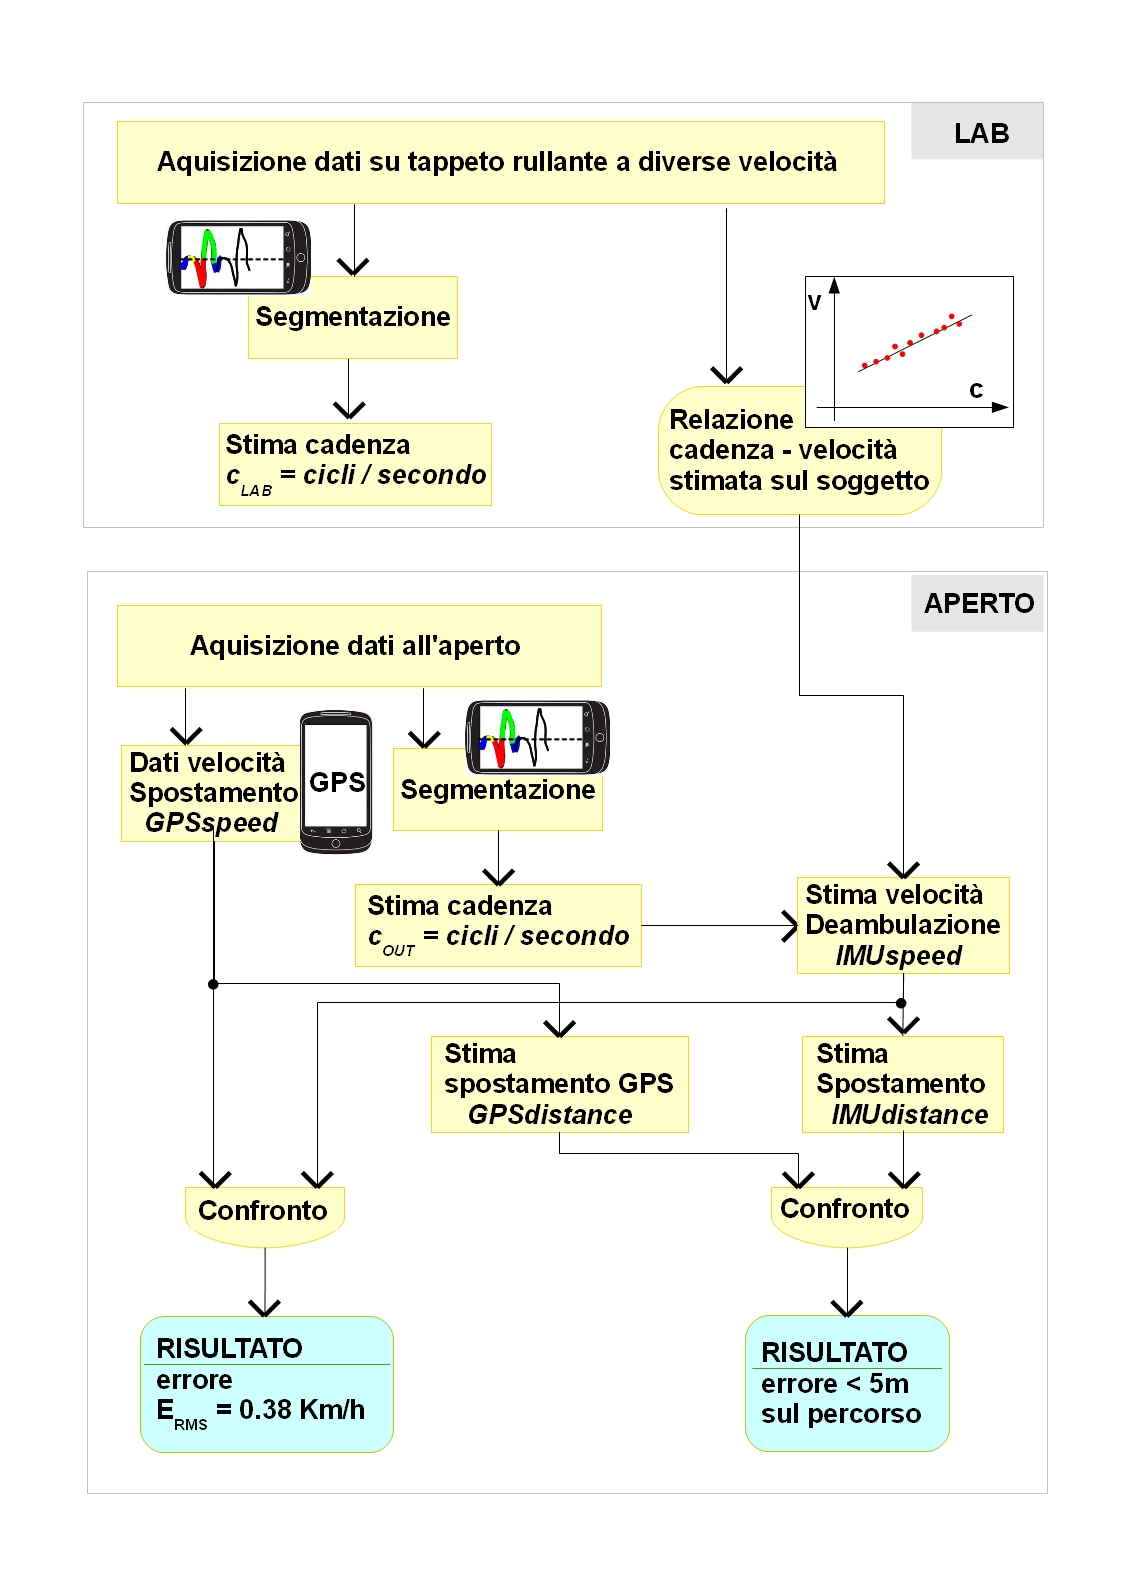
\includegraphics[width=1\textwidth]{imgs/ValutazionePrestazioniSistema.jpg}\\
\column{.5\textwidth}

\tiny{
\begin{table}[htbp]
		\centering
		\rowcolors{1}{RoyalBlue!20}{RoyalBlue!5}
		\begin{tabular}{l|c}
				\textbf{Attivit�}& cammino\\
				\textbf{Soggetti}& $1$\\
				\textbf{Velocit�}& $\{2,3,4,5,6,7,8\}\, km/h$\\
				\textbf{Durata}& $1:30\,minuti$  per attivit�\\
				\textbf{Strumenti} & IMU, Smartphone, tappeto rullante\\
				\textbf{Luogo}& Laboratorio\\
				\textbf{Dati raccolti} & valori giroscopio segmentati\\
				\textbf{Freq. camp.} & $100\,Hz$\\
			\end{tabular}
	\end{table}
}

\begin{flushleft}
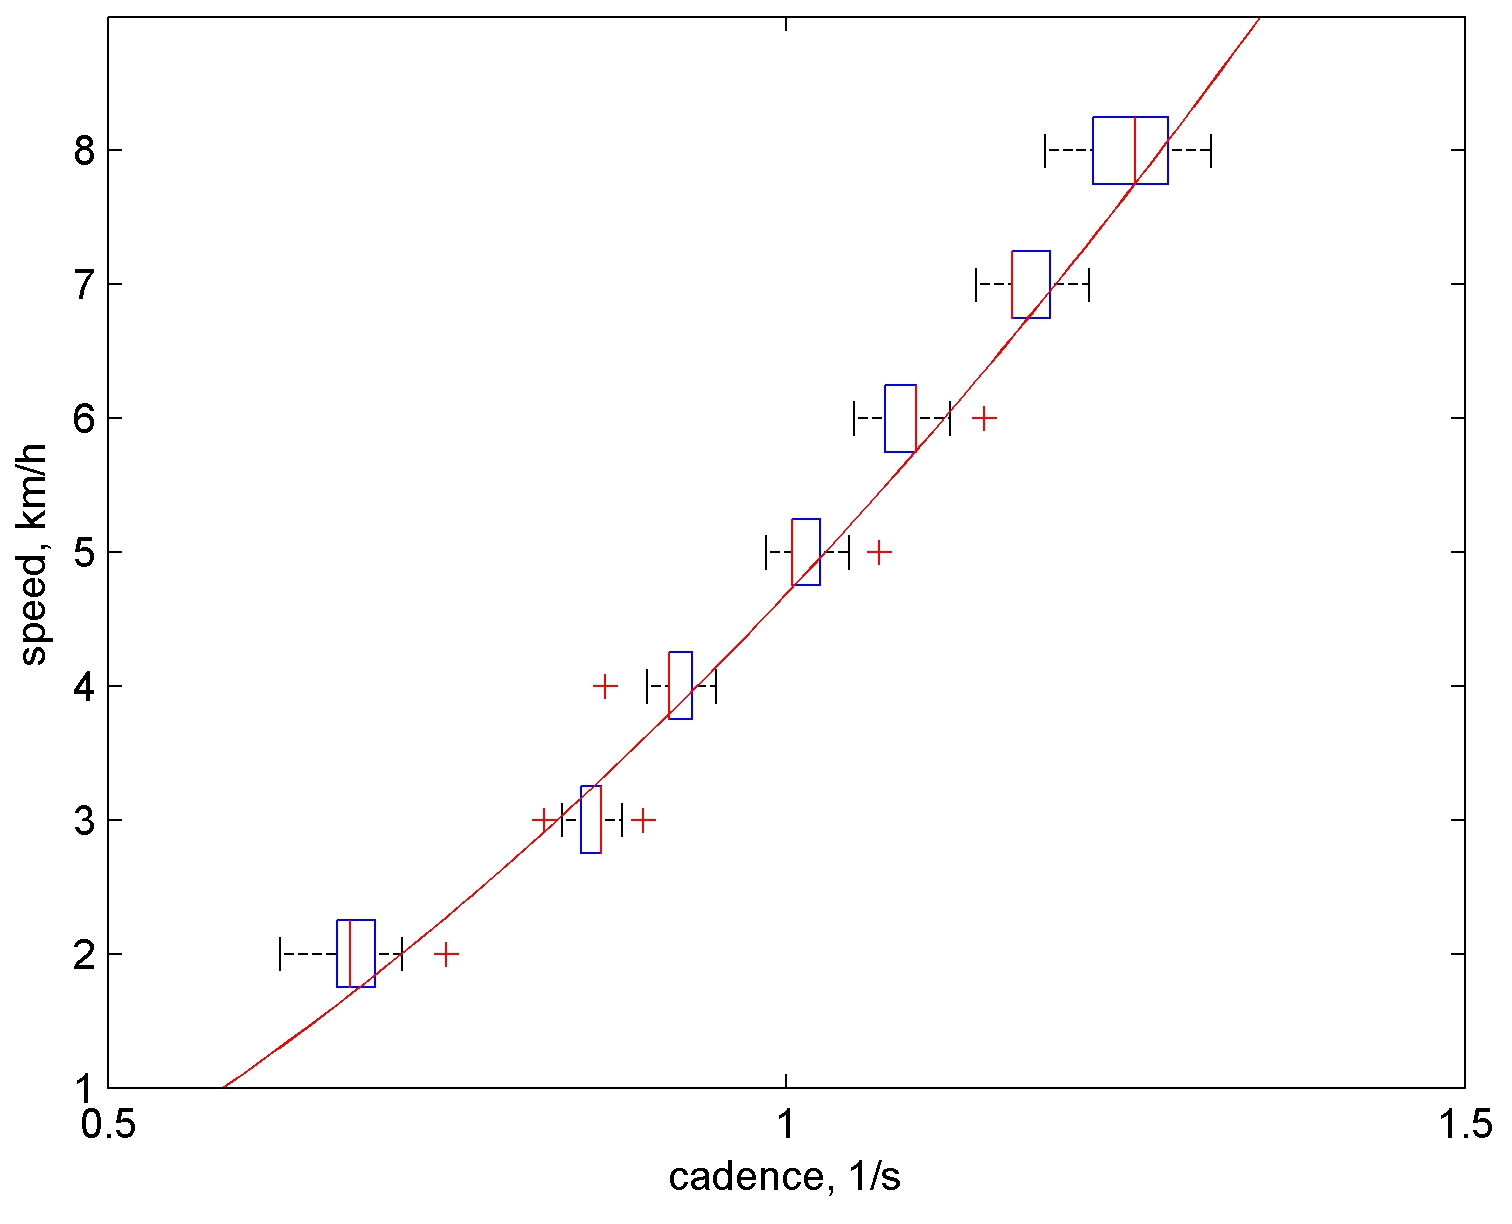
\includegraphics[width=1\textwidth]{imgs/cadVSspeed_boxplot.jpg}
\end{flushleft}

	
\end{columns}
}
